\documentclass[10pt]{extarticle}
\title{}
\author{Avinash Iyer}
\date{}
\usepackage[shortlabels]{enumitem}


%paper setup
\usepackage{geometry}
\geometry{letterpaper, portrait, margin=1in}
\usepackage{fancyhdr}

%symbols
\usepackage{amsmath}
\usepackage{amssymb}
\usepackage{amsthm}
\usepackage{mathtools}
\usepackage{hyperref}
\usepackage{gensymb}
\usepackage{multirow,array}

\newtheorem*{remark}{Remark}
\usepackage[T1]{fontenc}
\usepackage[utf8]{inputenc}

%chemistry stuff
%\usepackage[version=4]{mhchem}
%\usepackage{chemfig}

%plotting
\usepackage{pgfplots}
\usepackage{tikz}
\tikzset{middleweight/.style={pos = 0.5}}
\tikzset{weight/.style={pos = 0.5, fill = white}}
\tikzset{lateweight/.style={pos = 0.75, fill = white}}
\tikzset{earlyweight/.style={pos = 0.25, fill=white}}

%\usepackage{natbib}

%graphics stuff
\usepackage{graphicx}
\graphicspath{ {./images/} }
\usepackage[style=numeric, backend=biber]{biblatex} % Use the numeric style for Vancouver
\addbibresource{the_bibliography.bib}
%code stuff
%when using minted, make sure to add the -shell-escape flag
%you can use lstlisting if you don't want to use minted
%\usepackage{minted}
%\usemintedstyle{pastie}
%\newminted[javacode]{java}{frame=lines,framesep=2mm,linenos=true,fontsize=\footnotesize,tabsize=3,autogobble,}
%\newminted[cppcode]{cpp}{frame=lines,framesep=2mm,linenos=true,fontsize=\footnotesize,tabsize=3,autogobble,}

%\usepackage{listings}
%\usepackage{color}
%\definecolor{dkgreen}{rgb}{0,0.6,0}
%\definecolor{gray}{rgb}{0.5,0.5,0.5}
%\definecolor{mauve}{rgb}{0.58,0,0.82}
%
%\lstset{frame=tb,
%	language=Java,
%	aboveskip=3mm,
%	belowskip=3mm,
%	showstringspaces=false,
%	columns=flexible,
%	basicstyle={\small\ttfamily},
%	numbers=none,
%	numberstyle=\tiny\color{gray},
%	keywordstyle=\color{blue},
%	commentstyle=\color{dkgreen},
%	stringstyle=\color{mauve},
%	breaklines=true,
%	breakatwhitespace=true,
%	tabsize=3
%}
% text + color boxes
\usepackage[most]{tcolorbox}
\tcbuselibrary{breakable}
\newtcolorbox{problem}[1]{colback = white, title = {#1}, breakable}
\newtcolorbox{solution}{colback = white, colframe = black!75!white, title = Solution, breakable}
%including PDFs
%\usepackage{pdfpages}
\setlength{\parindent}{0pt}
\usepackage{cancel}
\pagestyle{fancy}
\fancyhf{}
\rhead{Avinash Iyer}
\lhead{Econ 305: Problem Set 3}
\newcommand{\card}{\text{card}}
\newcommand{\ran}{\text{ran}}
\newcommand{\N}{\mathbb{N}}
\newcommand{\Q}{\mathbb{Q}}
\newcommand{\Z}{\mathbb{Z}}
\newcommand{\R}{\mathbb{R}}
\begin{document}
  \begin{problem}{Strategies}
    Imagine an extensive-form game in which player $i$ has $K$ information sets.
    \begin{enumerate}[(a)]
      \item If the player has an identical number $m$ possible actions in each information set, how many pure strategies do they have?
      \item If the player has $m_k$ actions in information set $k\in \{1,2,\dots,K\}$, how many pure strategies does the player have?
    \end{enumerate}
    \tcblower
    \begin{problem}{(a)}
      The player has $mK$ strategies.
    \end{problem}
    \begin{problem}{(b)}
      The player has $\prod_{k=1}^{k}m_k$ pure strategies.
    \end{problem}
  \end{problem}
  \begin{problem}{A Beginner's Guide to Subgame Perfection}
    Consider the following extensive form game:
    \begin{center}
      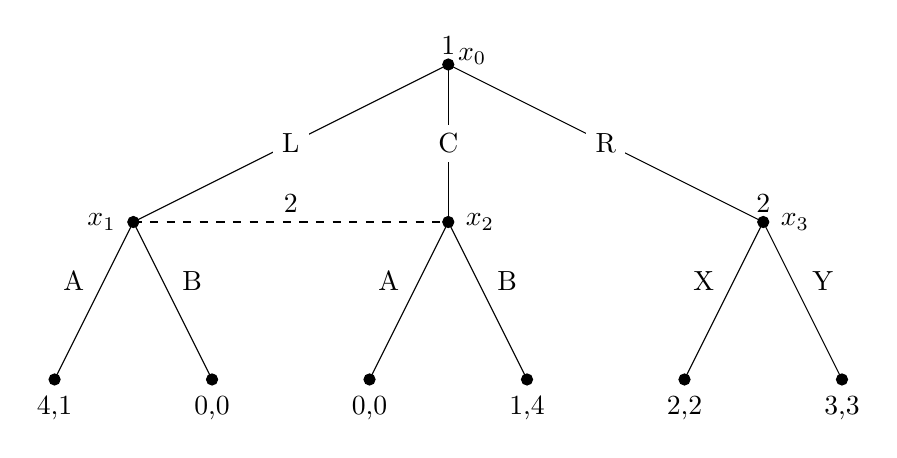
\begin{tikzpicture}
        \filldraw (0,0) circle(2pt)
              (-4,-2) circle (2pt)
              (0,-2) circle (2pt)
              (4,-2) circle (2pt)
              (-5,-4) circle (2pt)
              (-3,-4) circle (2pt)
              (-1,-4) circle (2pt)
              (1,-4) circle (2pt)
              (3,-4) circle (2pt)
              (5,-4) circle (2pt);
        \draw (0,0) -- node[middleweight,fill=white]{L} (-4,-2);
        \draw (0,0) -- node[middleweight,fill=white]{C} (0,-2);
        \draw (0,0) -- node[middleweight,fill=white]{R} (4,-2);
        \draw[dashed] (-4,-2) --node[middleweight,anchor=south]{2}(0,-2);
        \draw (-4,-2) -- node[middleweight,anchor = south east]{A} (-5,-4);
        \draw (-4,-2) -- node[middleweight,anchor = south west]{B}(-3,-4);
        \draw (0,-2) -- node[middleweight,anchor = south east]{A} (-1,-4);
        \draw (0,-2) -- node[middleweight,anchor = south west]{B}(1,-4);
        \draw (4,-2) -- node[middleweight,anchor = south east]{X} (3,-4);
        \draw (4,-2) -- node[middleweight,anchor = south west]{Y}(5,-4);
        \node[anchor = south] at (0,0){1};
        \node[anchor=west] at (0,0.1){$x_0$};
        \node[anchor = east] at (-4.1,-2){$x_1$};
        \node[anchor = west] at (0.1,-2){$x_2$};
        \node[anchor = west] at (4.1,-2){$x_3$};
        \node[anchor = south] at (4,-2){2};
        \node[anchor = north] at (-5,-4.1){4,1};
        \node[anchor = north] at (-3,-4.1){0,0};
        \node[anchor = north] at (-1,-4.1){0,0};
        \node[anchor = north] at (1,-4.1){1,4};
        \node[anchor = north] at (3,-4.1){2,2};
        \node[anchor = north] at (5,-4.1){3,3};
      \end{tikzpicture}
    \end{center}
    \tcblower
    \begin{problem}{(a)}
      Characterize the information sets of the decision nodes (denoted by $x_i$) in this game by writing down all the information sets for each player.
      \tcblower
      \begin{itemize}
        \item Player 1: $\{x_0\}$
        \item Player 2: $\{x_1,x_2\},\{x_3\}$
      \end{itemize}
    \end{problem}
    \begin{problem}{(b)}
      Write the normal-form game associated with this extensive form game and find all the pure strategy Nash equilibria.
    \end{problem}
    \begin{problem}{(c)}
      Which of the Nash equilibria that you found in part (b) are also subgame perfect equilibria?
    \end{problem}
  \end{problem}
  \begin{problem}{The Shipping News}
    Consider the following extensive form games. In both games, UPS ($U$) has to decide whether to Enter ($E$) or stay out ($O$) of a foreign market where DHL ($D$) is already active. If UPS enters the market, then both firms have to decide whether or not to start a price war by fighting $(F,F^*,f)$ or acquiescing $(A,A^*,a)$ to the entry. The payoffs list that of UPS first, followed by the payoff to DHL.
    \begin{center}
      \begin{tikzpicture}
        \filldraw (0,0) circle (2pt)
                  (-2,-2) circle (2pt)
                  (2,-2) circle (2pt)
                  (0,-4) circle (2pt)
                  (4,-4) circle (2pt)
                  (-1,-6) circle (2pt)
                  (1,-6) circle (2pt)
                  (3,-6) circle (2pt)
                  (5,-6) circle (2pt);
        \draw (0,0) --node[middleweight,anchor=south east]{$O$} (-2,-2);
        \draw (0,0) --node[middleweight,anchor = south west]{$E$} (2,-2);
        \draw (2,-2) --node[middleweight,anchor = south east]{$a$} (0,-4);
        \draw (2,-2) --node[middleweight,anchor = south west] {$f$} (4,-4);
        \draw (0,-4) --node[middleweight, anchor=south east]{$A$} (-1,-6);
        \draw (0,-4) --node[middleweight,anchor = south west]{$F$} (1,-6);
        \draw (4,-4) --node[middleweight, anchor = south east]{$A^*$} (3,-6);
        \draw (4,-4) --node[middleweight,anchor = south west]{$F^*$} (5,-6);
        \node[anchor = south] at (0,0.1) {$U$};
        \node[anchor = south] at (2,-1.9) {$D$};
        \node[anchor = west] at (4.1,-4) {$U$};
        \node[anchor = east] at (-0.1,-4) {$U$};
        \node[anchor = north] at (-2,-2) {0,5};
        \node[anchor = north] at (-1,-6) {1,2};
        \node[anchor = north] at (1,-6) {0,-3};
        \node[anchor = north] at (3,-6) {-3,1};
        \node[anchor = north] at (5,-6) {-2,-1};
      \end{tikzpicture}\\
      \begin{tikzpicture}
        \filldraw (0,0) circle (2pt)
                  (-2,-2) circle (2pt)
                  (2,-2) circle (2pt)
                  (0,-4) circle (2pt)
                  (4,-4) circle (2pt)
                  (-1,-6) circle (2pt)
                  (1,-6) circle (2pt)
                  (3,-6) circle (2pt)
                  (5,-6) circle (2pt);
        \draw (0,0) --node[middleweight,anchor=south east]{$O$} (-2,-2);
        \draw (0,0) --node[middleweight,anchor = south west]{$E$} (2,-2);
        \draw (2,-2) --node[middleweight,anchor = south east]{$a$} (0,-4);
        \draw (2,-2) --node[middleweight,anchor = south west] {$f$} (4,-4);
        \draw (0,-4) --node[middleweight, anchor=south east]{$A$} (-1,-6);
        \draw (0,-4) --node[middleweight,anchor = south west]{$F$} (1,-6);
        \draw (4,-4) --node[middleweight, anchor = south east]{$A^*$} (3,-6);
        \draw (4,-4) --node[middleweight,anchor = south west]{$F^*$} (5,-6);
        \draw[dashed] (0,-4) -- node[middleweight,anchor = south]{$U$}(4,-4);
        \node[anchor = south] at (0,0.1) {$U$};
        \node[anchor = south] at (2,-1.9) {$D$};
        \node[anchor = north] at (-2,-2) {0,5};
        \node[anchor = north] at (-1,-6) {1,2};
        \node[anchor = north] at (1,-6) {0,-3};
        \node[anchor = north] at (3,-6) {-3,1};
        \node[anchor = north] at (5,-6) {-2,-1};
      \end{tikzpicture}
    \end{center}
    \tcblower
    \begin{problem}{(a)}
      What is the difference between the two extensive form games with respect to what the players know when they make their decisions?
      \tcblower
      In the first game, UPS only makes its decision to acquiesce or fight after DHL does, but in the second game, UPS and DHL make their decision simultaneously.
    \end{problem}
    \begin{problem}{(b)}
      Write the normal form of both games and find all of the pure strategy Nash equilibria in each game.
    \end{problem}
    \begin{problem}{(c)}
      Find all subgame perfect equilibria of both games.
    \end{problem}
  \end{problem}
\end{document}
